%%  USB-TPLE
%%  Flyer für Embedded World 2010
%% 
%%  Andreas Müller, andz@gmx.de
%%  2010-02-26
%% 
\def\filename{flyer.tex}
\def\fileversion{v1.1}   % change this when leaflet-manual changed, too.
\def\filedate{2014/01/01}
\def\docdate {2014/01/01} % change this when leaflet-manual changed, too.
\listfiles
\errorcontextlines=99
\documentclass[
a4paper,
%%notumble,
%%nofoldmark,
%%dvipdfm,
%%portrait,
%%titlepage,
%%nocombine,
%%a3paper,
%%debug,
%%nospecialtricks,
%%draft,
]{leaflet}


\renewcommand*\foldmarkrule{.3mm}
\renewcommand*\foldmarklength{5mm}

\usepackage[T1]{fontenc}
\usepackage{textcomp}
\usepackage{mathptmx}
\usepackage[scaled=0.9]{helvet}
\makeatletter
\def\ptmTeX{T\kern-.1667em\lower.5ex\hbox{E}\kern-.075emX\@}
\DeclareRobustCommand{\ptmLaTeX}{L\kern-.3em
        {\setbox0\hbox{T}%
         %\vb@xt@ % :-)
         \vbox to\ht0{\hbox{%
                            \csname S@\f@size\endcsname
                            \fontsize\sf@size\z@
                            \math@fontsfalse\selectfont
                            A}%
                      \vss}%
        }%
        \kern-.12em
        \ptmTeX}
\makeatother
\let\TeX=\ptmTeX
\let\LaTeX=\ptmLaTeX
\usepackage{shortvrb}
\MakeShortVerb{\|}
\usepackage{url}
\usepackage{graphicx}
\usepackage[dvipsnames,usenames]{color}
\usepackage[ngerman]{babel}
\definecolor{LIGHTGRAY}{gray}{.9}
\definecolor{FHOrange}{rgb}{1.0,0.4,0.0}

%%%%\renewcommand{\descfont}{\normalfont}
\newcommand\Lpack[1]{\textsf{#1}}
\newcommand\Lclass[1]{\textsf{#1}}
\newcommand\Lopt[1]{\texttt{#1}}
\newcommand\Lprog[1]{\textit{#1}}

\newcommand*\defaultmarker{\textsuperscript\textasteriskcentered}

\newcommand{\changefont}[3]{ \fontfamily{#1} \fontseries{#2} \fontshape{#3} \selectfont}

\renewcommand{\familydefault}{\sfdefault}
\usepackage{helvet}

\title{USB-TPLE}
\author{
  Andreas M\"uller, HS-Augsburg\\
  \\
  Prof. Dr. Hubert H\"ogl, HS-Augsburg}


%%\CutLine*{1}% Dotted line without scissors
\CutLine*{6}%  Dotted line without scissors

\AddToBackground{5}{%  Background of a small page
  \put(0,0){\textcolor{FHOrange}{\rule{\paperwidth}{\paperheight}}}}

\AddToBackground{6}{%  Background of a small page
  \put(0,0){\textcolor{FHOrange}{\rule{\paperwidth}{\paperheight}}}}



\begin{document}

%%\maketitle
%%\thispagestyle{empty}

%%\LARGE

%%\tableofcontents

\changefont{pag}{m}{n}


\begin{flushright}


\includegraphics [scale=0.2]{logo.png}

\end{flushright}

\begin{center}

\vskip 40pt

\Huge Logikanalyse \linebreak f"ur Alle\\


\bigskip

\vskip 30pt



\vskip 30pt

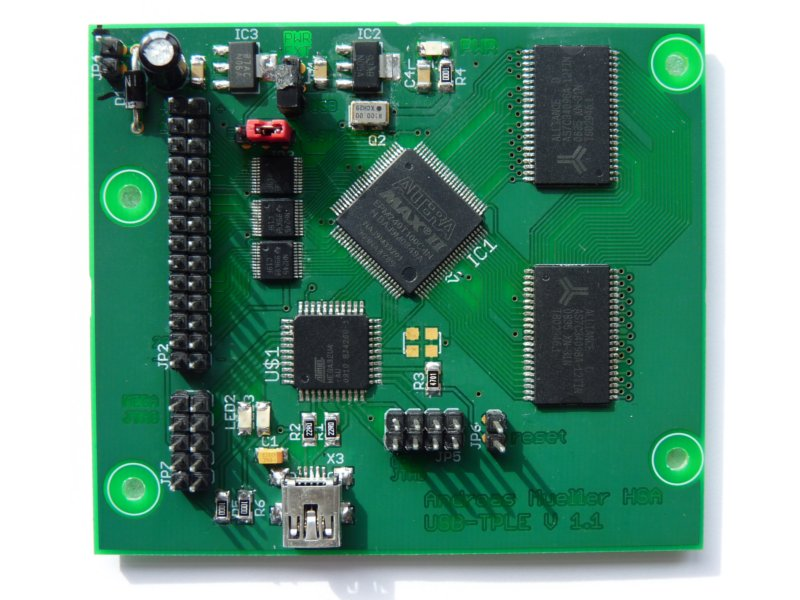
\includegraphics {board.jpg}

\vskip 30pt

\Large Ein universelles, rekonfigurierbares und freies USB Ger\"at zur Timing-, Protokoll-, Logik- und Eventanalyse von digitalen Signalen
\end{center}

\eject

\section{\"Ubersicht}

Hauptaufgabe des Projektes ist die Erfassung und Aufzeichnung des zeitlichen Verlaufs von digitalen Signalen und Ereignissen. So kann zum Beispiel an einem Mikrocontroller ohne Beeinflussung der Laufzeit die Dauer eines Prozesses oder die Zustandsfolge an den Pins "uber die Zeit gemessen werden. Auch eine Protokollanalyse digitaler Busse wie I2C oder SPI ist mit dem Logikanalysator m"oglich.

Kernst"uck des Systems ist ein konfigurierbarer Logikbaustein (CPLD) der Firma Altera, sowie ein Mikrocontroller der Firma Atmel mit USB Anbindung. 

Das gesamte Projekt, sowohl Hard- als auch Software, ist im Sinne von Open-Source frei verf"ugbar. Ein TRAC mit SVN Repository kann unter der URL

{\bf \underline \tt \large https://io.informatik.fh-augsburg.de/trac/Logikanalysator}

abgerufen werden.


\section{Funktionen}

Hauptfunktion ist, wie oben beschrieben, die Logikanalyse an Mikrocontrollern. Dazu wird zum Beispiel zu Beginn und zum Ende eines Prozesses ein Assemblerbefehl gesetzt, welcher einen Impuls auf einem IO Port des Mikrocontrollers ausgibt. Der Zeitpunkt des Impulses kann durch das Ger"at auf bis zu 0.16 Mikrosekunden genau aufgezeichnet werden.

Aufgrund der komplett freien Konfigurierbarkeit der Hardware sind jedoch auch weitere Anwendungen wie Protokoll- und Logikanalyse sowie auch ein Logikgenerator implementierbar.

\section{Eigenschaften}

\begin{itemize}
  \item 8 Kan"ale
  \item Abtastung mit bis zu 6,25 MSamples/s
  \item Aufl"osung maximal 160ns
  \item Speicher f"ur bis zu 262144 Samples
  \item Stromversorgung "uber Jumper einstellbar (USB/ext.)
  \item Messpannung w"ahlbar (3.3V/5.0V)
  \item Einfache Ansteuerung "uber USB
  \item Firmware Update von Mikrocontroller und CPLD per USB
  \item Anbindung an sigrok und gtkwave
\end{itemize}

\section{Hardware}

\subsection{Prozessor}

Als CPU kommt ein Mikrocontroller der Firma Atmel zum Einsatz. Der ATMEGA32U4 ist ein Controller der 8-Bit AVR Serie mit den folgenden Eigenschaften:

\begin{itemize}
  \item 32KB Flashspeicher
  \item 2.5KB RAM
  \item Integrierte USB Schnittstelle
  \item Bootloader (Konfigurierbar "uber USB)
\end{itemize}

Die Software f"ur den Mikrocontroller ist in C geschrieben und basiert auf LUFA, einem USB-Framework f"ur AVR Mikrocontroller. Die Kommunikation mit dem CPLD erfolgt "uber einen 4-Bit breiten synchronen Datenbus.

\subsection{CPLD}

Als Logikbaustein wird ein Low-Cost CPLD der Firma Altera verwendet. Der CPLD der MAX II Serie ist mit 100MHz getaktet und "uber einen 16-Bit breiten Datenbus mit einem externen, schnellen RAM verbunden. Als Hardwarebeschreibungssprache kommt VHDL zum Einsatz und als Synthesetool wird das kostenlose Quartus II der Herstellerfirma verwendet.

\begin{itemize}
  \item 240 Logikzellen
  \item Konfigurierbar "uber JTAG oder direkt durch den Mikrocontroller
  \item 24 IO Ports f"ur Messungen verf"ugbar; Aktuell werden nur 8 IO Ports verwendet
\end{itemize}

\subsection{Speicher}

Auf dem Prototypen befinden sich zwei \linebreak Speicherbausteine mit jeweils 256K*16 Bit. Bei einer Messung wird der aktuelle logische Zustand der Messeing"ange bei einer "Anderung in den Speicher geschrieben. Zus"atzlich wird ein Zeitstempel und ein Statusbyte zur "Uberpr"ufung der G"ultigkeit einer Messung gespeichert. Die Messdaten und das Statusbyte ben"otigen  jeweils 8 Bit und der Zeitstempel 16 Bit. F"ur eine Messung werden also 32 Bit ben"otigt. Somit k"onnen bis zu 262.144 Ereignisse aufgenommen werden. Wenn die Messung abgeschlossen ist, kann der Mikrocontroller die aufgezeichneten Messwerte vom CPLD abfragen und an den PC weiterreichen.

\section{Software}

Gesteuert werden kann das System mit jedem beliebigen Terminalprogramm "uber eine virtuelle serielle Schnittstelle.

Die Speicherung erfolgt "uber das Value-Change-Dump-Format. Dieses, auf ASCII basierende Format f"ur Logiksignale, vereint zwei wesentliche Vorteile. Es ist eine problemlose Nutzung "uber ein Terminal m"oglich und das Open Source Programm GTK-Wave ist zu diesem Dateiformat kompatibel.

Es ist geplant, die Signal-Analyse Software sigrock als grafisches Frontend f"ur die Steuerung des USB-TPLE zu verwenden. Sigrock ist eine Open-Source Software und kann auf verschiedenen Plattformen wie zum Beispiel Linux, Windows verwendet werden. Es ist allerdings eine Erweiterung n"otig, um die Hardware richtig ansteuern zu k"onnen.

\section{Entwicklungsstatus}

Im Jahr 2010 wurde von Andreas M"uller ein erster funktionsf"ahiger Prototyp der Hardware in seiner Bachelorarbeit "{}USB-TPLE - ein universelles, rekonfigurierbares und freies USB Ger\"at zur Timing-, Protokoll-, Logik- und Eventanalyse von digitalen Signalen"{} entwickelt. Im Rahmen einer Technischen Projektarbeit (f"unftes Semester Technische Informatik) wurde f"ur den bestehenden Prototypen eine Firmware sowohl f"ur den CPLD als auch f"ur den Mikrocontroller entwickelt. Auch eine PC-Software, mit der der Benutzer die Hardware bedienen kann, ist entstanden. Es hat sich herausgestellt, dass die 240 im CPLD verf"ugbaren Logikelemente f"ur komplexere Aufgaben nicht ausreichen. Deshalb wird f"ur weitere Entwicklungen ein CPLD mit mehr Logikzellen n"otig sein. 

Der aktuelle Status kann auf der Projektseite eingesehen werden:

\vskip 30pt

\begin{center}
{\bf \underline \tt \large https://io.informatik.fh-augsburg.de/trac/Logikanalysator}
\end{center}

\eject

\vspace*{\fill}




{\bf \underline \tt Technische Projektarbeit (WS 2013/14):}

Andreas Gareis\\Stefan Vockinger\\Matthias Weber\\Bernd Krafft\\Patrick Echter\\Nils Bunje

{\bf \underline \tt Projektbetreuer:}

Prof. Dr. Hubert H\"ogl

Hochschule Augsburg\\https://io.informatik.fh-augsburg.de/trac/Logikanalysator

{\bf \underline\tt Bachelorarbeit "{}USB-TPLE"{} (2010):}

Andreas M"uller

%%\endgroup
\end{document}

%%
%% End of file `leaflet-manual.tex'.
